\section{Proteins}
\subsection{Amino Acids \& Poly-Peptides}
Proteins are the mechanism by which
executive function takes place in the cell. 
This is includes the implementation
of activities such as \emph{"metabolism, growth,
architecture and regulation of cell and organism"} -\cite{lesk}.
Proteins themselves are composed
of discrete molecular units termed amino acids, the precise
way in which they amino acids arrange themselves is dependent
of the genetic sequence of the parent organism itself.
There exist 20 unique amino acids (examples given below) that can be combined
that can be sequenced into strings of 
arbitrary length of any order following chemical laws.
\begin{table}
    \begin{center}
        \caption{}
\begin{tabular}{||c | c||}
    \hline
    \multicolumn{2}{||c||}{Examples of proteins and their codes}\\
    \hline\hline
    Glycine & G  \\ 
    \hline
    Alanine & A \\
    \hline
    Serine & S  \\
    \hline
    Cysteine & C  \\
    \hline
    Threorine & T \\ 
    \hline
    Proline & P \\
    \hline
    Valine &  V\\
    \hline
    Leucine & K \\ [1ex] 
    \hline
\end{tabular}
\end{center}
\end{table}
These molecules come together to form peptide bonds,
this occurs when the carboxyl group ($^-COOH$) bonds to the
\emph{amino} group ($^+NH_3$) of another amino acid producing 
water as a by-product of the reaction \cite{lesk}.
\begin{figure}
    \caption{Peptide Bond}
    \includesvg{Figures/PeptideBond} 
    \scriptsize{\dag Image Source: \url{https://en.wikipedia.org/wiki/Peptide_bond}}
\end{figure}
Despite all amino acids possessing an amino and
carboxyl group, every amino acid has a unique side chain,
an additional molecular group attached to the main chain.
The unique chemical properties of these side chains are responsible
for the interactions in that molecule's \emph{neighbourhood};
a term that is expanded on in the next few sections.

\subsection{Protein Structures}
\begin{figure}[!htb]
    \caption{Structure of a peptide unit}
    \begin{center}
        \chemfig{-[1]C_{\beta_{i-1}}(=[2]O)-N_i(-[1]C_{\alpha_i}(-[2]C_{\beta_{i}})(-[7]C_{\beta_{i+1}}(=[6]O)(-[1])))}
    \end{center}
\end{figure}

The carbon atom that joins the side chain to
the main chain is denoted as the $\alpha$ carbon
atom and the carbon atoms in immediate contact with the
$\alpha$ carbons are known as $\beta$ 
 carbons\footnote{In figure 2.2 subscript $i$ denotes membership to a unique unit}. The bond angles between the $C_{\alpha_i} - C_{\beta_i+1}$
 and $C_{\alpha_i} - N_i$ groups are commonly denoted
 as $\psi$ and $\phi$ respectively. Stereochemically
 feasible angles can be described by a Ramachandran plot as in figure 2.3. \\

 \begin{figure}[!htb]
    \caption{Ramachandran plot}
    \begin{center}
        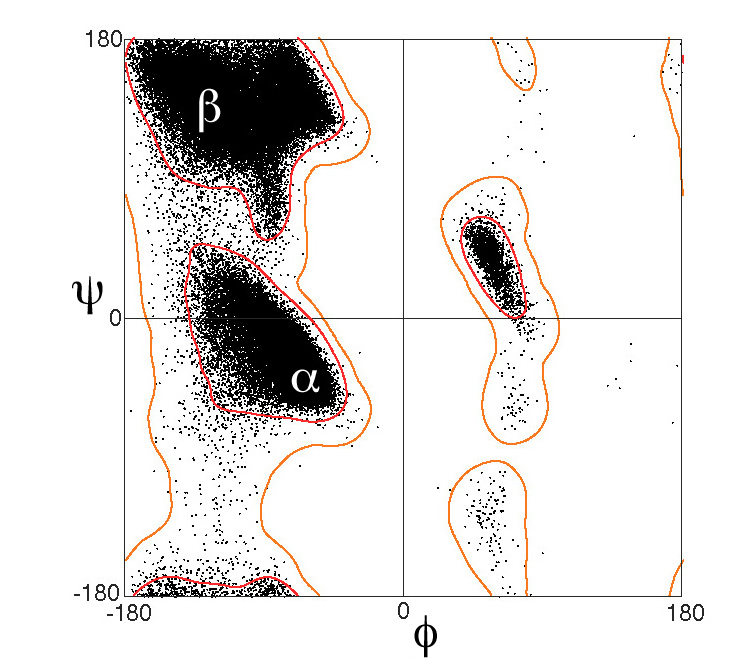
\includegraphics[scale=0.6]{Figures/RamachandranPlot}
    \end{center}
    \scriptsize{\dag Source: \url{https://proteopedia.org/wiki/index.php/Ramachandran_Plots}}
 \end{figure}
Poly-peptide conformations can be described by three structures:

\begin{enumerate}
    \item \textbf{Primary Structure} \\
        This is the encoding of a protein as a 1-D sequence
        of its constituent amino acids. \\I.e:
        \[DTYGYWEPYT\]
    \item \textbf{Secondary Structure} \\
        This encoding represents local, repeating structures
        with respect to the entire conformations. These
        structures satisfy chemical restraints common to most proteins\footnote{The hydrogen bonding potential of main-chain $N-H$ and $C=O$ groups \cite{lesk}}.
        In particular, the formation of structures known as $\alpha$\footnote{$B$ in fig 2.4} helices
        and $\beta$\footnote{$E$ in fig 2.4} sheets largely facilitate the energetic 
        and conformational constraints imposed by the interactions
        amongst the side-chains orthogonal to the backbone. These
        structures form the dense regions in the Ramachandran plot.
    \item \textbf{Tertiary Structure} \\
        A protein's tertiary structure are its 3D atomic
        coordinates in space. The protein's torsion backbone
        (main-chain) traces out a curve through space parameterised
        by all pairs $(\phi, \psi)$ for each residue pair. Hydrogen bonds, which arise when neighbouring residues are in close
        proximity although not directly connected by the backbone, hold together the various secondary structures in specific
        conformations such that the global energy of the system is 
        minimized \cite{Yang}.
\end{enumerate}
\begin{figure}[!htb]
    \caption{Secondary and tertiary structures}
    \begin{center}
        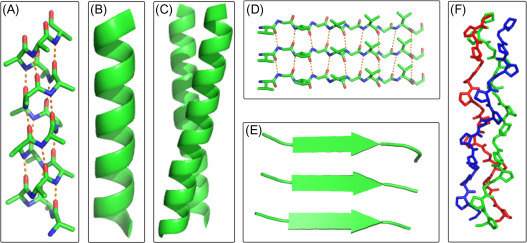
\includegraphics[scale=0.8]{Figures/Structures}
    \end{center}
    \scriptsize{\dag Source: \cite{Boyle}}
 \end{figure}
 The primary goal of protein structure prediction
 is the \emph{ab initio} determination of a protein's
 tertiary structure from its primary structure \cite{Yang}
 which can be described as a mapping:
 \begin{equation}
    \mathbf{X}^n \coloneqq \text{Set of all sequences of length $n$}
 \end{equation}
 \begin{equation}
    \mathbf{F}:\mathbf{X}^n \rightarrow ((\phi,\psi)_1 \ldots (\phi,\psi)_n)
 \end{equation}
 \cite{Anfinsen} et al showed that the protein's
 tertiary structure is entirely encoded by 
 its primary structure; the implications of this are explored next.

\subsection{The Protein's Energy Landscape}
Due in part to the continuous spectrum of stereochemically 
plausible values of $(\phi, \psi)$, the possible number of conformations
for a given sequence are extraordinarily large. 
Given that each possible conformation has an associated free energy,
Levinthal's paradox states that if all conformations were equally
energetically favourable, then protein would essentially have to undergo
a random walk along the \emph{Gibbs free energy} surface until it has found its native conformation.
The free energy surface in this respect refers to the manifold that is formed
by taking the \emph{distribution} over conformations $((\phi, \psi)_1\ldots(\phi,\psi)_n)$ at every time-step
and $\Delta G$ at every point to form a surface in $2n+1$ dimensional space.
Given that common proteins have in the order of 100-1000+ constituent residues,
the combinatorial size of the state space would prohibit any efforts to find 
a specific conformation by random walk with vanishing probability. \\
\cite{Yang} address both the paradox and subsequent critiscisms;
part of their work can be summarised by the following lemmas:
\begin{lemma}
    Not all conformations are equally energetically favourable.
\end{lemma}
\begin{proof}
    Proteins fold spontaneously in the order of \emph{nanoseconds} into their native
    conformation in a solvent at constant temperature, thus they cannot
    be traversing the whole state space.
\end{proof}
\begin{lemma}
    There must therefore be a driving reaction that narrows down the search space.
\end{lemma}
\begin{proof}
    Folding appears to undergo two consecutive stages, tier 1
    occurs of a timescale of \emph{nanoseconds} and tier 2 appears
    to occur over a scale of \emph{picoseconds}, a reduction in 3
    orders of magnitude. Thus the peptide must undergo a slower
    interaction that constrains the state space followed by a final, 
    faster "relaxation" into the native state.
\end{proof}
\begin{lemma}
    By undergoing hydrophobic collapse,
    the remaining residues have restricted degrees of freedom,
    thus a reduced subspace consisting of
    only energetically feasible conformations is explored, 
    within this subspace there exists one unique solution whose
    energy is minimized.
\end{lemma}
\begin{proof}
    The relative timescales of the tier 1 and tier 2 interactions indicate
    a smooth slope in conformational space that greatly 
    constrains the possible conformations, followed by a 
    second tier of faster interactions that enables the system to
    quickly overcome the local maxima and minima 
    which gives way to the global optimum at the bottom of the subset.
\end{proof}
\begin{lemma}
    If there exists only one unique conformation whose Gibbs free energy
    is minimal amongst all possible conformations, the manifold must be
    "funnel shaped".
\end{lemma}
\begin{proof}
    The nature of the hydrophobic collapse
    "drops" the full state space into a smaller subspace,
    the unique global minimum lies within this subspace.
    If there existed more than one unique solution, then a given
    sequence could form into multiple possible native conformations, this
    would violate the marginal stability property of the native state
    so there cannot exist more than one unique solution. 
\end{proof}

\[ \Delta G = \Delta H - T \Delta S \]
By the second law of thermodynamics, the entropy (amount of disorder) in a closed system
can never decrease over time and can remain constant only if the
system is in equilibrium, thus a state of maximum entropy \cite{jaffe}.
The work of \cite{Yue,Yang} show that the overall increase in entropy
of the peptide-solvent system is primarily motivated by a phenomenon known as the
\emph{hydrophobic collapse} whereby all the water produced as by-product of the peptide bond
\footnote{See fig 2.1} "squeezes" the hydrophobic residues
into globular core. Following \textbf{Lemma 4}, the process appears
to be guided by a heuristic search in this subspace,
enabling it to swiftly reach its native state.\\

\begin{figure}[!htb]
    \caption{Gibbs free energy funnel}
    \begin{center}
        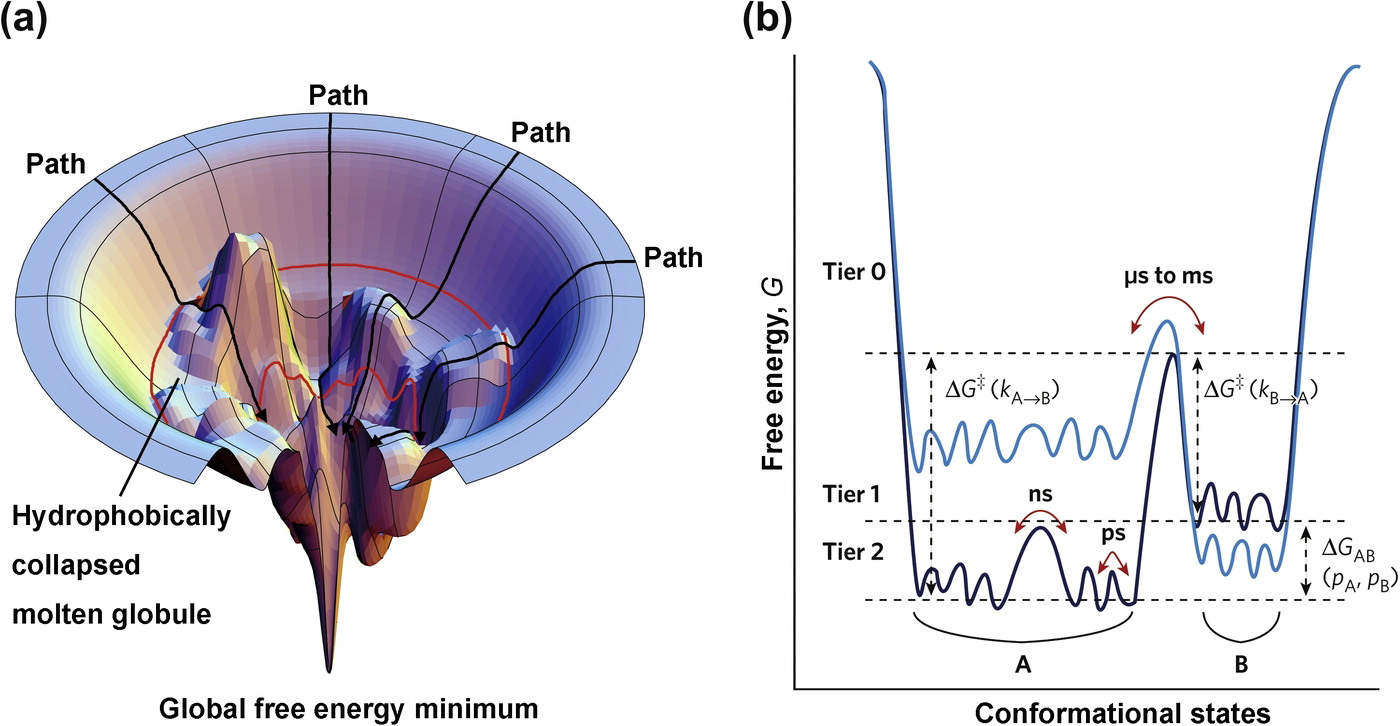
\includegraphics[trim={0 0 4cm 0.25cm},scale=1, clip]{Figures/FreeEnergyLandscape}
    \end{center}
    \scriptsize{\dag Source: \cite{Yang}}
 \end{figure}

Critically, the notion of $\Delta G$ is with respect to the distribution
over conformations, indicating that at any point the protein exists as an
ensemble of possible conformations, and the native state consists of a
collection of conformations whose joint distribution minimises the value of $\Delta G$.
I reformulate this property as maximum likelihood objective:
\begin{theorem}
    \
    \begin{enumerate}
        \item Let $T \in \mathbf{\{X\}}^n$ denote the native state as a tuple of $n$ torsion angles (follows from eq. 2.1).
        \item Let $P(\mathbf{F}(\mathbf{X}^n; \theta))$ denote the distribution over all
        functional mappings from a primary sequence to a tuple of $n$ torsion
        angles with parameters $\theta$ (follows from eq. 2.2).
    \end{enumerate}
    The search for a function that maps the protein's primary structure to its tertiary structure
    can be formulated as the maximization of the posterior probability
    that function $\mathbf{F}$ with parameters $\theta$ maps sequence $\mathbf{X}^n$ to state $T$.
    \begin{equation}
        P(T | \mathbf{F}(\mathbf{X}^n; \theta))\ =\frac{P(\mathbf{F}(\mathbf{X}^n; \theta) | T) \cdot P(T)}{P(\mathbf{F}(\mathbf{X}^n; \theta))}
    \end{equation}
\end{theorem}                                                                                                                                                                                                                                                     
This formulation is further explored in the \textbf{System Requirements and Specification}
section, however an interesting detail to note is that this is equivalent to sampling
the maximum likelihood estimate from the posterior of a \emph{Gaussian process} \footnote{See appendix A.1}.

\subsection{Bioinformatics}
There exists experimental techniques to determine the protein's
native (or \emph{crystalline}) structure\footnote{Such as X-Ray Crystallography \cite{Chayen}},
however these approaches are out of the scope of this
project and are not given a detailed analysis. Otherwise,
these techniques can often require years of trial and error 
and can be very costly \cite{alberts}.

In recent years, advancements in both hardware and processing power
have enabled computational methods to play increasingly significant role 
in the PSP problem. I will focus briefly what's known
as homology modelling as this is relevant to understanding related
supervised learning methods, and then I will then provide extended review
of another class of models used for \emph{ab initio} structure prediction,
lattice models.
\subsubsection{Homology Modelling}
All proteins are members of an evolutionary tree and so related
proteins tend to demonstrate high structural similarity with their relatives.
Although older studies suggest that proteins are in fact random strings
only slightly edited by evolution \cite{weiss}; more recent studies
have shown that this is not the case, as certain methods
were able to distinguish between random strings and real proteins
with an accuracy of up to $88-94.36\%$ \cite{delucrezia,Tsygvintsev}.
Given the apparent specificity of the sequences,
Homology modelling, focuses on trying to predict 
the tertiary structure of an unknown protein
from the structures of closely related proteins (homologues).
This involves measuring Hamming distances\footnote{See appendix A.2} 
between closely related proteins and deriving an \emph{inverse scoring matrix}
with each pair-wise comparison. When this is done for more than
one possible pairing, this is known as Multiple Sequence Alignment (MSA).
Highly correlated proteins with relatively low MSA scores tend to exhibit
very similar tertiary structures \cite{lesk}; this property is used as the basis for many
machine learning methods which is explored in \textbf{Related Work}.
\subsubsection{Lattice Models}
Although approaches that utilise homology modelling in some form
have been very successful in recent years\footnote{See \textbf{AlphaFold 2.4.2.1}},
they rely on the pre-determined structures of other proteins, this poses
a barrier to \emph{de novo} protein design and research into undetermined structures
for which we do not have a readily available dataset of relatives.

An alternative model of computation was proposed by \cite{Yue} that seeks to
address the combinatorial conformational space. Instead, they proposed
that the space should be discretised to restrict the possible number of conformations
a given sequence can take on, a \emph{Bravais} lattice was the perfect tool for this.
\subsubsection{Bravais Lattices}
A Bravais lattice is a simple mathematical description of a lattice structure, whereby
each point in space is some linear combination of unit vectors with integer multiples \cite{kittel}. 
\begin{center}
\begin{equation}
    \begin{split}
        & \mathbf{r}, \mathbf{a} \in \mathbb{R}^n, u \in \mathbb{Z} \\
        & \mathbf{r} = u_1\mathbf{a}_1 + u_2\mathbf{a}_2 + u_3\mathbf{a}_3 
    \end{split}
\end{equation}
    In matrix form:
\begin{equation}
    \begin{split}
        & \mathbf{r} \in \mathbb{R}^n, \mathbf{u} \in \mathbb{Z}^n \\
        & \mathbf{a} \in \mathbb{R}^n \times \mathbb{R}^n \\
        & \mathbf{r} = \mathbf{a} \cdot \mathbf{u}^\top
    \end{split}
\end{equation}
\end{center}
Different values for the unit vectors give rise to different classes of lattices, the number
of neighbours for a given vertez is denoted as $z$.
In the interest of brevity 3 lattices are discussed as they are pertinent 
to the related work and system design. \\
\begin{enumerate} 
    \item \textbf{2D Square Lattice} \\ 
        A simple lattice whose unit vectors are two dimensional: 
        \begin{equation}
            \begin{split}
                & \mathbf{a} = \begin{bmatrix}
                    1 & 0 \\
                    0 & 1
                    \end{bmatrix} \\
                & z = 4
            \end{split}
        \end{equation}
    \item \textbf{3D Primitive Cubic Lattice} \\
        A 3D lattice with unit vectors in each direction of space:
        \begin{equation}
            \begin{split}
               & \mathbf{a} = \begin{bmatrix}
                1 & 0 & 0 \\
                0 & 1 & 0 \\
                0 & 0 & 1
            \end{bmatrix} \\
            & z = 6 
            \end{split}
        \end{equation}
    \item \textbf{3D Face-Centered Cubic Lattice} \\
        A 3D cubic lattice with additional vertex points
        at the center of each square face; notably,
        this lattice has the highest sphere packing density \footnote{Highest amount
        of rigid spheres that can be packed per unit space $\approx 0.74$ \cite{Hoque}}:
        \begin{equation}
            \begin{split}
                & \mathbf{a} = \begin{bmatrix}
                    0 & 0.5 & 0.5 \\
                    0.5 & 0 & 0.5 \\
                    0.5 & 0.5 & 0
                \end{bmatrix} \\
                & z = 12
            \end{split}
        \end{equation}
\end{enumerate}

\begin{figure}[!htb]
    \caption{3D Cubic Bravais Lattices}
    \begin{center}
        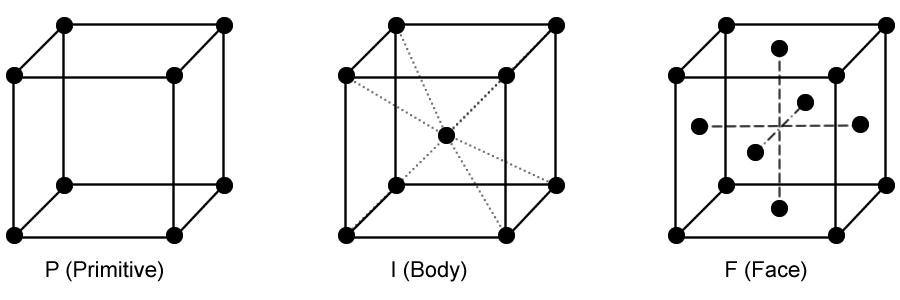
\includegraphics[scale=0.25]{Figures/lattices}
    \end{center}
    \scriptsize{\dag Source: \url{https://biochem.co/2008/08/crystal-structure-studies/}}
 \end{figure}
 For clarity, any point within the vector space defined by the lattice
 structure is an integer multiple of any linear combination of the unit vectors. Nomenclature
 on the subject dictates that a vertex on the lattice is 
 referred to as a "\emph{site}". 
\subsubsection{HP Model}
\cite{Yue} initially proposed the use of a 3D primitive cubic lattice to model the conformations
of proteins. Each amino acid was divided into two categories according to their properties:
Hydrophobic and Polar, and a conformation was formulated as a self avoiding walk (SAW) on the lattice.
\\ Some definitions:
\begin{itemize}
    \item A \emph{contact} on the lattice is define as the adjacency of two immediate neighbours on the lattice
    not connected by the torsion backbone, if two residues are connected 
    through the torsion backbone directly this is referred to 
    as a \emph{bond}.
    \item A segment is a run of monomers of a particular category (a)\footnote{P segment of length 4}, a singlet
          occurs when a monomer is situated between two monomers of another category (b)\footnote{H singlet}.

    \begin{multicols}{2}
        \noindent
        \begin{align*}
            \underset{(a)}{HPPPPH} 
        \end{align*}
        \begin{align*}
            \underset{(b)}{PHP}
        \end{align*}
    \end{multicols}
    \item $x \in \{H,P\}$
    \item $n_x$ is the number of $x$ monomers in the sequence. \\
        I.e: $n_H$ is the number of $H$ monomers in the entire sequence.
    \item $b_{xx}$ is number of bonds between $xx$.
    \item $t_{xx}$ is the number of \emph{bonds + contacts} between $xx$.
    \item $h_{term}$ is the number of segements that terminate in $H$ monomers
\end{itemize}
These quantities are related by the following equations:
\begin{equation}
    2b_{HH} + b_{HP} + h_{term} + (z-2)n_H = 2(t_{HH} + b_{HH}) + b_{HP} + t_{HP} + t_{H-Solvent}
\end{equation}
\begin{equation}
    \begin{split}
        & G = \frac{b_{HP} + h_{term}}{2} \\
        & S = b_{HP} + t_{HP} + t_{H-Solvent} \\
    \end{split}
\end{equation}
\begin{itemize}
    \item $G$ is the total number of $H$ segments in a sequence
    \item $S$ is the total surface area of the hydrophobic core, assuming that
        the monomers as \textbf{unconnected}. This acts as an upper bound of the surface
        area.
\end{itemize}

Substituting (2.10) into (2.9) produces the \emph{"folding equation"}:
\begin{equation}
    t_{HH} + \frac{S}{2} = G + \frac{(z-2)n_H}{2}
\end{equation}
Where the left side is dependent on the \emph{conformation}, and the right
side is a constant that solely depends on the lattice structure and given sequence.
Motivated by the role of the hydrophobic collapse, the folding problem within this
framework is a function that maximises $t_{HH}$ ; this is equivalent to
minimizing $S$. The logic follows that the most tightly packed core, that with the minimal
surface area should also have the densest packing of $H-H$ contacts. \\
\subsubsection{hHPNX Model}
